%----------------------------------------------------------------------------------------
%	PACKAGES AND THEMES
%----------------------------------------------------------------------------------------
\documentclass[aspectratio=169,xcolor=dvipsnames,handout]{beamer}
\usetheme{Darmstadt}
\usecolortheme{seahorse}

\usepackage[hangul]{kotex}

\usepackage{hyperref}
\usepackage{graphicx} % Allows including images
\usepackage{booktabs, multicol, multirow} % Allows the use of \toprule, \midrule and \bottomrule in tables
\setbeamercovered{transparent}
%----------------------------------------------------------------------------------------
%	TITLE PAGE
%----------------------------------------------------------------------------------------

\title[공공선택 이론]{공공선택 이론} % The short title appears at the bottom of every slide, the full title is only on the title page
\subtitle{경제정의와 불평등}

\author[오성재]{오성재}

\institute[HNU] % Your institution as it will appear on the bottom of every slide, may be shorthand to save space
{
    한남대학교 \\
    탈메이지 교양학부 \\
}
\date{\today} % Date, can be changed to a custom date


%----------------------------------------------------------------------------------------
%	PRESENTATION SLIDES
%----------------------------------------------------------------------------------------

\begin{document}

\begin{frame}
    % Print the title page as the first slide
    \titlepage
\end{frame}

\begin{frame}{목차}
    % Throughout your presentation, if you choose to use \section{} and \subsection{} commands, these will automatically be printed on this slide as an overview of your presentation
    \tableofcontents
\end{frame}
%------------------------------------------------


\begin{frame}[<+->]
\frametitle{공공선택이론(Public Choice Theory)}
    \begin{itemize}
       \item<1-> 주요 주제 :  불가능성 정리는 모든 가능한 형태의 선호를 다룬다는 점에서 어려움.
       \item<2-> 주요 주제 :  제한된 형태의 선호를 다룬다면 효율적이면서 민주적인 사회후생함수.
       \item<3-> 주요 주제 : 
       \begin{enumerate}
           \item<4> 집단의사결정 과정의 성격.
           \item<5> 집단의사결정에서 파생되는 자원배분상의 함의.
           \item<6> 정부의 행태에 대한 예측과 설명.
       \end{enumerate} 
   \end{itemize}
\end{frame}
%------------------------------------------------
%------------------------------------------------
\section{직접민주제하의 공공선택}
%------------------------------------------------

\begin{frame}{투표제도의 특성}
    \begin{itemize}[<+->]
        \item 표 배정방식 : 1인 1표, 점수투표, 주주총회 의결권, 특별의결권(UN 안보리 거부권) 등등.
        \item 투표방식 : 1회 투표제, 다회 투표제(결선 투표제) 등등.
        \item 의사결정조건 :  전원합의제, (가중)과반수제  등등.
    \end{itemize}
\end{frame}
%------------------------------------------------

\begin{frame}{전원합의제(Unanimity)}
    \begin{itemize}[<+->]
        \item 만장일치제.
        \item 장점
        \begin{itemize}
            \item 파레토 효율적.
        \end{itemize}
        \item 단점
        \begin{itemize}
            \item 의안도출의 어려움.
            \item 전략적 거부.
            \item 현재상태({\it status quo})의 우월성.
        \end{itemize}
        \item 중요사안에 대하여 소수를 대상으로 사용 가능.
    \end{itemize}
\end{frame}
%------------------------------------------------

\begin{frame}{과반수제(Majority rule)}
    \begin{itemize}[<+->]
        \item 과반수 찬성으로 통과.
        \item 장점
        \begin{itemize}
            \item 단순함.
            \item 합의 도출이 가능.
        \end{itemize}
        \item 단점
        \begin{itemize}
            \item 다수의 횡포(tyranny of the majority).
            \item 투표의 역설(voting paradox).
        \end{itemize}
    \item 중요 사안에 대하여 가중투표($2/3$ 또는 $3/4$)로 보완.
    \end{itemize}
\end{frame}
%------------------------------------------------
\begin{frame}
    \begin{itemize}
        \item 가중투표는 대안의 결정을 어렵게 한다.
    \end{itemize}
    \begin{columns}
        \begin{column}{.5\textwidth}
            \begin{figure}
                \centering
                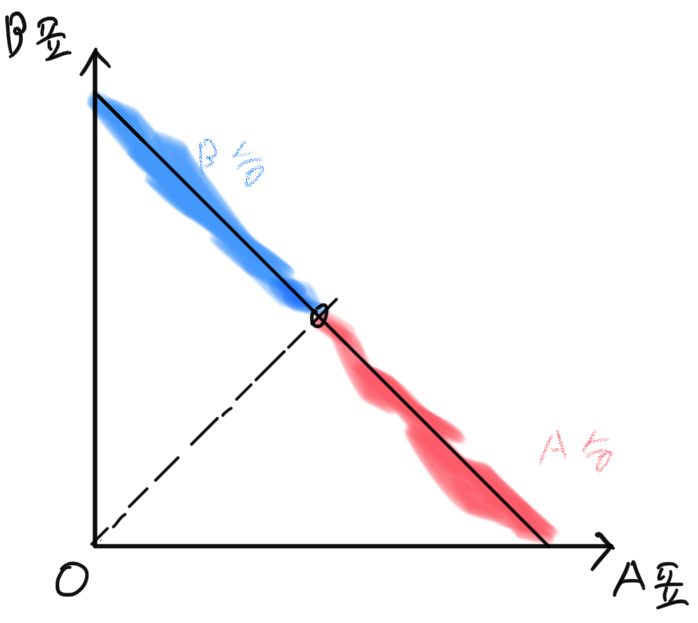
\includegraphics[scale=.2]{pic/onehalf.png}
                \caption{과반수제}
            \end{figure}
        \end{column}    
        \begin{column}{.5\textwidth}
            \begin{figure}
                \centering
                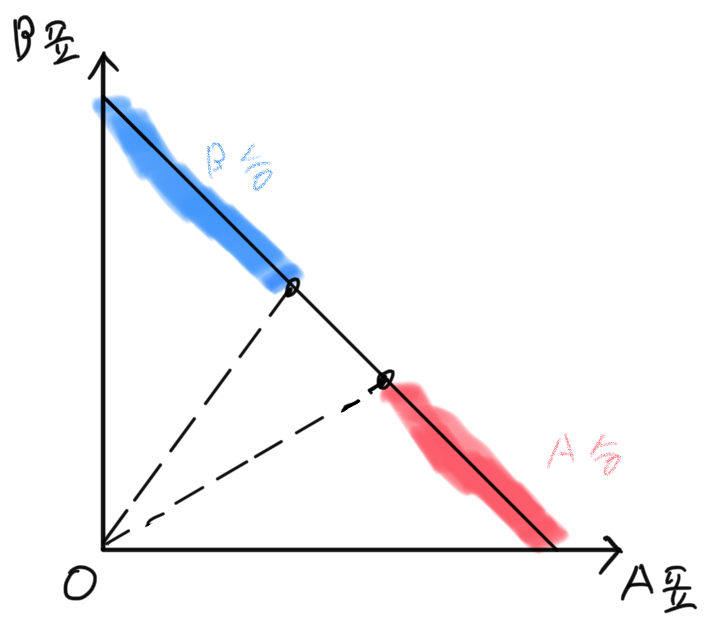
\includegraphics[scale=.2]{pic/twothird.png}
                \caption{$2/3$ 가중다수제}
            \end{figure}
        \end{column}    
    \end{columns}
\end{frame}
%------------------------------------------------

\begin{frame}{점수투표제(Point Voting)}
    \begin{itemize}[<+->]
        \item 1인 1표제의 경우 선호의 강도를 표현할 방법이 없음.
        \item 투표자에게 일정 점수를 주고 스스로 점수를 배정하게 함.
        \item 전략적 행위(voting strategy)에 취약함.
    \end{itemize}
    \pause
    \begin{table}
        \centering
        \begin{tabular}{c|c|c|c|c|c|c|c}
            \toprule
                          & 투표자1 & 투표자2 & 투표자3 & 투표자4 & 투표자5 & 투표자6 & 합계 \\
            \hline 후보 A & 6 & 4 & 5 & 7 & 0 & 1 & 23 \\
                   후보 B & 3 & 3 & 3 & 2 & 7 & 1 & 19 \\
                   후보 C & 1 & 3 & 2 & 1 & 3 & 8 & 18 \\
            \bottomrule
        \end{tabular}
        \caption{점수투표제 하의 전략적 행위}
    \end{table}
\end{frame}
%------------------------------------------------

%------------------------------------------------
\section{과반수제하에서의 정치적 균형}
%------------------------------------------------


\begin{frame}{중위투표자 이론(median voter theorem)I}
    \begin{itemize}[<+->]
        \item 사람 $ = \{X, Y, Z \}$.
        \item 대안 $ = \{A, B, C \}$.
        \item 투표방식 : 두 대안씩 과반수 투표. 선택 못받은 대안은 탈락. 한 개의 대안이 남을 때 까지 반복.
        \item {\bf 꽁도세승자(Condorcet winner)}: 위의 투표에서 살아남은 최후의 대안.
    \end{itemize}
    \begin{block}{중위투표자 이론(median voter theorem)}
      셋 이상의 대안에 대하여 모든 투표자들이 단봉선호를 가진다고 가정하자. 이때 {\bf 중위투표자(median voter)}가 존재하고 그가 선호하는 대안이 투표로 선택된다. 
    \end{block}
\end{frame}

\begin{frame}{중위투표자론II}
    \begin{columns}
        \begin{column}{.5\textwidth}<1->
            \begin{table}[]
                \begin{tabular}{cc}
                     X: & A $\succ$ B $\succ$ C \\
                     Y: & C $\succ$ B $\succ$ A \\
                     Z: & B $\succ$ C $\succ$ A
                \end{tabular}
                \caption{개인들의 선호}
            \end{table}
        \end{column}
        \begin{column}{.5\textwidth}<2>
            \begin{figure}
                \centering
                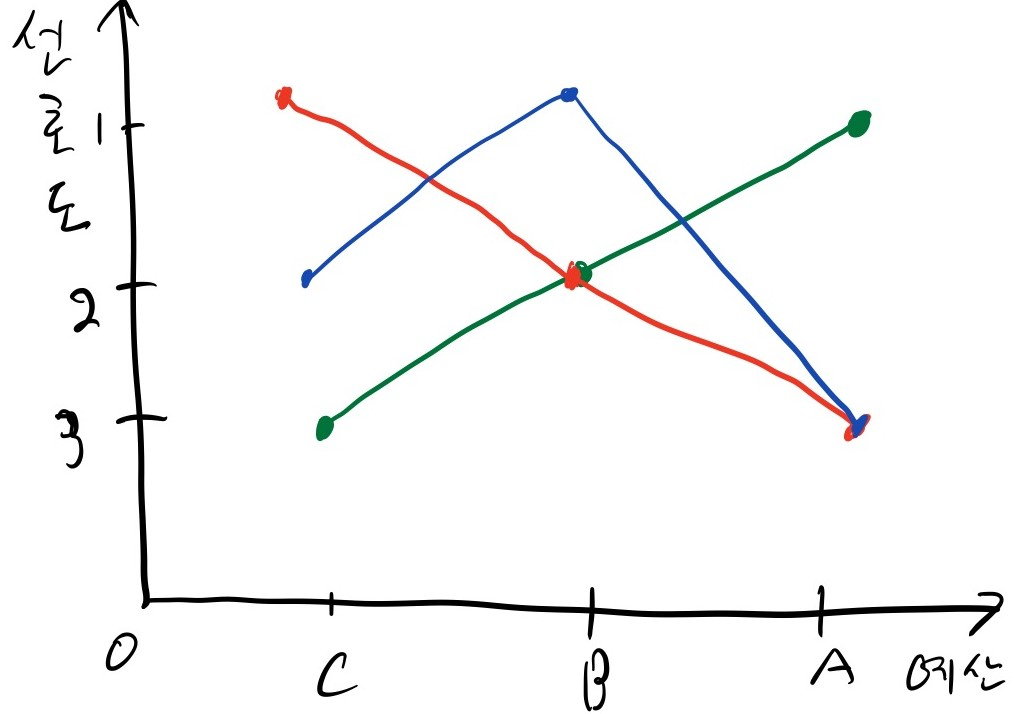
\includegraphics[width=.8\textwidth]{pic/voting1.jpg}
                \caption{개인들의 선호}
            \end{figure}
        \end{column}
    \end{columns}
\end{frame}
%------------------------------------------------

\begin{frame}{투표의 역설(Voting Paradox)I}
    \begin{itemize}[<+->]
        \item 투표자 선호의 분포에 순환(cycling)이 있을 경우, 비교 순서가 결과에 영향.
        \item {\bf 의사진행조작(agenda manipulation)}을 통해 결과를 조작.
    \end{itemize}
\end{frame}
%------------------------------------------------

\begin{frame}{투표의 역설II}
    \begin{columns}
        \begin{column}{.5\textwidth}<1->
            \begin{table}[]
                \begin{tabular}{cc}
                     X: & A $\succ$ B $\succ$ C \\
                     Y: & B $\succ$ C $\succ$ A \\
                     Z: & C $\succ$ A $\succ$ B
                \end{tabular}
                \caption{개인들의 선호}
            \end{table}
        \end{column}
        \begin{column}{.5\textwidth}<2>
            \begin{figure}
                \centering
                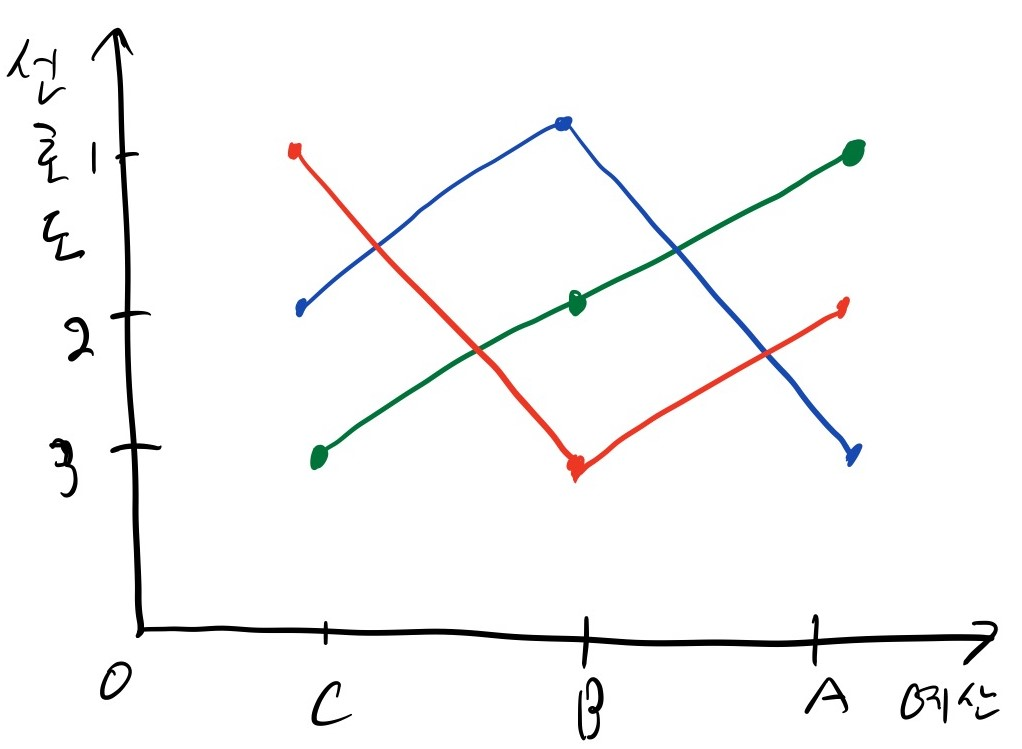
\includegraphics[width=.8\textwidth]{pic/voting2.jpg}
                \caption{개인들의 선호}
            \end{figure}
        \end{column}
    \end{columns}
\end{frame}
%------------------------------------------------

\begin{frame}{투표의 역설의 원인}
    \begin{itemize}[<+->]
        \item {\bf 다봉선호(multi-peak-preference)}
        \begin{itemize}
            \item 공공서비스 vs. 민간서비스 예산배정.
            \item 다차원적 대안.
        \end{itemize}
        \item {\bf 단봉선호(single-peak-preference)}
        \begin{itemize}
            \item 투표의 역설이 일어나지 않음.
            \item 소비자 선호의 볼록성(convex preference).
            \item 고정된 가격.
        \end{itemize}
    \end{itemize}
\end{frame}
%------------------------------------------------

\begin{frame}{단봉선호의 예 }
    \begin{figure}
        \centering
        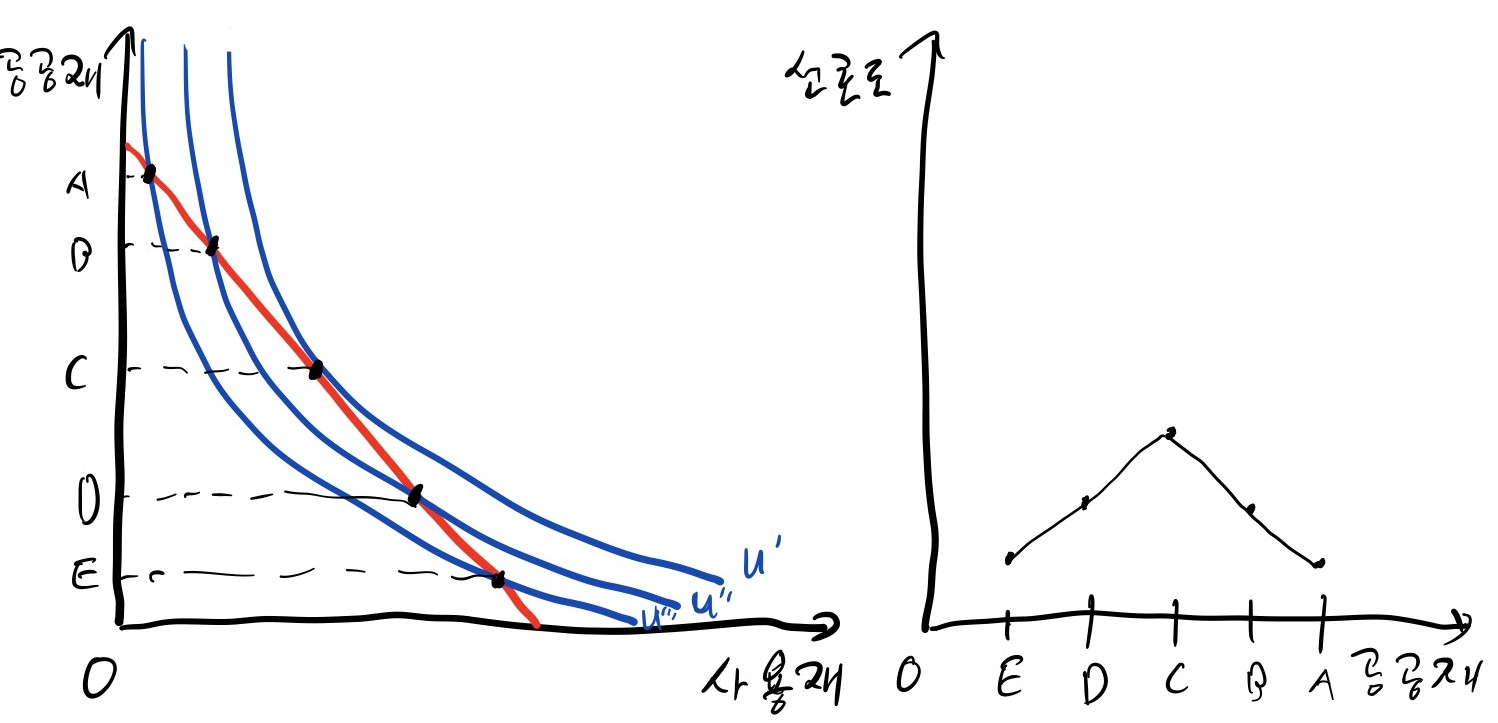
\includegraphics[width=.7\textwidth]{pic/singlepeak.jpg}
        \caption{선호의 볼록성과 단봉선호}
    \end{figure}
\end{frame}
%------------------------------------------------

\begin{frame}
\frametitle{투표의 불가능성 정리(Gibbard-Satterswaite theorem)}
    \begin{block}{투표불가능성 정리} 
        어떤 투표제도가 셋 이상의 대안에 대하여 비독재성을 가진다고 하자. 이 제도는 전략적 선택에 취약하다.
    \end{block}
    \begin{itemize}
        \item 전략적 선택 : 투표자가 자신의 진실된 선호가 아닌 투표를 할때 더 나은 결과를 가져오는 행위.
    \end{itemize}
\end{frame}
%------------------------------------------------

%------------------------------------------------
\section{대의민주제하의 공공선택}
%------------------------------------------------

\begin{frame}{논의의 배경}
    \begin{itemize}
        \item 대의민주제하에서 정부의 주요 주체들에 대한 행태를 분석.
        \begin{itemize}
            \item 정치가, 관료, 특수이익집단.
        \end{itemize}
        \item 각자의 이득을 추구하는 경제주체.
        \begin{itemize}
            \item 사익추구 가정의 비현실성.
            \item 사익추구 행위가 반드시 사회적 비효율을 야기하는 것은 아님.
        \end{itemize}
    \end{itemize}
\end{frame}
%------------------------------------------------
\subsection{정치가}

\begin{frame}{정치가}
    \begin{itemize}
        \item 표 극대화 모형(voting maximization theory)
        \begin{itemize}
            \item 투표자는 자신의 이익을 극대화.
            \item 정치가는 표를 극대화 하기 위한 정책 추진.
            \item 중위투표자가 선호하는 방향으로 정책 결정.
        \end{itemize}
    \end{itemize}
\end{frame}
%------------------------------------------------
\begin{frame}{호텔링 모형(Hotelling model)}
    \begin{itemize}
        \item 대안은 숫자 0과 1 사이의 실수 대표. 
        \item 투표자들은 0과 1 사이에 단봉선호를 가지고 고르게 분포.
        \item 대안은 중위투표자와 가깝게 위치하려고 함.
    \end{itemize}
\end{frame}
%------------------------------------------------

\begin{frame}{투표자 연합}
    \begin{itemize}[<+->]
        \item 개별 의안에 대해 견해를 달리하는 투표자들이 서로 연합하여 공동의 이익을 추구할 수 있음.
        \item 개별 투표자들의 연합은 정치가들이 정강(platform)의 형태로 구현.
    \end{itemize}
    \pause
    \begin{table}
        \centering
        \begin{tabular}{cc|c|c|c|c|c|c}
            \toprule
            \multicolumn{2}{c|}{\multirow{2}{*}{의안}} & \multicolumn{6}{c}{투표자} \\
                     \cline{3-8} & & A & B & C & D & E & 합계 \\
            \hline \multirow{2}{*}{1.징병제} & 존속 & 0 & 6 & 4 & 6 & 6 & 22  \\
                     & 폐지 & 10 & 4 & 6 & 4 & 4 & 28  \\
            \hline \multirow{2}{*}{2.가족법} & 존속 & 4 & 4 & 4 & 6 & 9 & 27  \\
                     & 폐지 & 6 & 6 & 6 & 4 & 1 & 23  \\
            \bottomrule
        \end{tabular}
        \caption{의안별 연합에 대한 투표자의 선호 예시}
    \end{table}
\end{frame}
%------------------------------------------------

\begin{frame}{정치적 결탁}
    \begin{itemize}
        \item 투표자들이 직접 연합해 표를 주고 받는 행위.
        \item 긍정적 평가
        \begin{itemize}
            \item 자발적인 표의 교환은 효율적 집단의사결정을 가능하게 하는 행위.
            \item 정치적 타협의 구체화.
        \end{itemize}
        \item 부정적 평가
        \begin{itemize}
            \item 특정 집단의 의사가 전체의사로 왜곡.
            \item 매표, 야합 등 부정적 결과 야기.
        \end{itemize}
    \end{itemize}
\end{frame}
%------------------------------------------------
\subsection{관료}

\begin{frame}[<+->]
\frametitle{관료}
    \begin{itemize}
        \item 예산극대화(budget maximization)
        \item 도덕적헤이(moral hazard)
        \item 형식주의(red tape)
        \item 위험기피(risk-aversion)성향
    \end{itemize}
\end{frame}
%------------------------------------------------
\subsection{특수이해집단}

\begin{frame}[<+->]
\frametitle{특수이해집단}
    \begin{itemize}
        \item 소수의 순편익이 다수의 순편익보다 적어도 특수집단의 이익대로 대안이 선택된다.
        \item 특수집단의 종류
        \begin{itemize}
            \item 산업별 집단 : 에너지, 반도체 등등.
            \item 직능별 집단 : 기업인, 노동자 등등.
            \item 주제별 집단 : 소비자운동, 환경운동 등등.
        \end{itemize}
    \end{itemize}
    
\end{frame}
%------------------------------------------------
%----------------------------------------------------------------------------------------

\end{document}
